%   terminology:
%     process: refers to execution in user space, or maybe struct proc &c
%     process memory: the lower part of the address space
%     process has one thread with two stacks (one for in kernel mode and one for
%     in user mode)
% talk a little about initial page table conditions:
%     paging not on, but virtual mostly mapped direct to physical,
%     which is what things look like when we turn paging on as well
%     since paging is turned on after we create first process.
%   mention why still have SEG_UCODE/SEG_UDATA?
%   do we ever really say what the low two bits of %cs do?
%     in particular their interaction with PTE_U
%   sidebar about why it is extern char[]

\chapter{Operating system organization}
\label{CH:FIRST}

A key requirement for an operating system is to support several activities at once.  For
example, using the system call interface described in
Chapter~\ref{CH:UNIX}
a process can start new processes with 
\lstinline{fork}.
The operating system must 
\indextext{time-share} 
the resources of the computer among these processes.
For example, even if there are more processes
than there are hardware CPUs, the operating
system must ensure that all of the processes
get a chance to execute.  The operating system must also arrange for
\indextext{isolation} 
between the processes.
That is, if one process has a bug and malfunctions,
it shouldn't affect processes that
don't depend on the buggy process.
Complete isolation, however, is too strong, since it should be possible for
processes to intentionally interact; pipelines are an example.
Thus
an operating system must fulfill three requirements: multiplexing, isolation,
and interaction.

This chapter provides an overview of how operating systems are
organized to achieve these three requirements.  It turns out there are
many ways to do so, but this text focuses on mainstream designs
centered around a \indextext{monolithic kernel}, which is used by many
Unix operating systems.  This chapter also provides an overview of an
xv6 process, which is the unit of isolation in xv6, and the
creation of the first process when xv6 starts.

Xv6 runs on a \indextext{multi-core}\footnote{
By ``multi-core'' this text means multiple CPUs that share memory but execute
in parallel, each with its own set of registers.
This text sometimes uses the term
\indextext{multiprocessor} as a synonym for multi-core,
though multiprocessor can also refer more specifically to a computer with
several distinct processor chips.} RISC-V microprocessor,
and much of its low-level
functionality (for example, its process implementation) is specific to
RISC-V.  RISC-V is a 64-bit CPU, and xv6 is written in ``LP64'' C,
which means long (L) and pointers (P) in the C programming language
are 64 bits, but int is 32-bit.  This book assumes the reader has done
a bit of machine-level programming on some architecture, and will
introduce RISC-V-specific ideas as they come up.  A useful reference
for RISC-V is ``The RISC-V Reader: An Open Architecture
Atlas''~\cite{riscv}.
The user-level ISA~\cite{riscv:user} and the privileged
architecture~\cite{riscv:priv} are the official
specifications.

The CPU in a complete computer is surrounded by support hardware, much
of it in the form of I/O interfaces. Xv6 is written for the support
hardware simulated by qemu's ``-machine virt'' option. This includes
RAM, a ROM containing boot code, a serial connection to the user's
keyboard/screen, and a disk for storage.

%% 
\section{Abstracting physical resources}
%% 

The first question one might ask when encountering an operating system is why
have it at all?  That is, one could implement the system calls in
Figure~\ref{fig:api}
as a library, with which applications link.  In this plan,
each application could even have its own library tailored to its needs.
Applications could directly interact with hardware resources
and use those resources in the best way for the application (e.g., to achieve
high or predictable performance).  Some operating systems for
embedded devices or real-time systems are organized in this way.

The downside of this library approach is that, if there is more than one
application running, the applications must be well-behaved.
For example, each application must periodically give up the
CPU so that other applications can run.
Such a 
\textit{cooperative} 
time-sharing scheme may be OK if all applications trust each
other and have no bugs. It's more typical for applications
to not trust each other, and to have bugs, so one often wants
stronger isolation than a cooperative scheme provides.

To achieve strong isolation it's helpful to forbid applications from
directly accessing sensitive hardware resources, and instead to abstract the
resources into services.  For example, Unix applications interact with storage
only through the file system's
\lstinline{open},
\lstinline{read},
\lstinline{write}, 
and
\lstinline{close}
system calls,
instead of reading and writing the disk directly. 
This provides the application with the convenience of pathnames, and it allows
the operating system (as the implementer of the interface) to manage the disk. 
Even if isolation is not a concern,
programs that interact intentionally (or just wish to keep
out of each other's way) are likely to find a file system a more convenient
abstraction than direct use of the disk.

Similarly, Unix transparently switches hardware CPUs among processes,
saving and restoring register state as necessary,
so that applications don't have to be
aware of time sharing.  This transparency allows the operating system to share
CPUs even if some applications are in infinite loops.

As another example, Unix processes use 
\lstinline{exec}
to build up their memory image, instead of directly interacting with physical
memory.  This allows the operating system to decide where to place a process in
memory; if memory is tight, the operating system might even store some of
a process's data on disk.
\lstinline{Exec}
also provides
users with the convenience of a file system to store executable program images.  

Many forms of interaction among Unix processes occur via file descriptors.
Not only do file descriptors abstract away many details (e.g.,
where data in a pipe or file is stored), they are also defined in a
way that simplifies interaction.
For example, if one application in a pipeline fails, the kernel
generates an end-of-file signal for the next process in the pipeline.

The system-call interface in
Figure~\ref{fig:api}
is carefully designed to provide both programmer convenience and
the possibility of strong isolation.  The Unix interface
is not the only way to abstract resources, but it has proven to be a very good
one.

%% 
\section{User mode, supervisor mode, and system calls}
%% 

Strong isolation requires a hard boundary between applications and the operating
system.  If the application makes a mistake, we don't want the operating system
to fail or other applications to fail. Instead, the operating system should be
able to clean up the failed application and continue running other applications.
To achieve strong isolation, the operating system must arrange that applications cannot modify (or even
read) the operating system's data structures and instructions and that
applications cannot access other processes' memory.

CPUs provide hardware support for strong isolation.   For
example, RISC-V has three modes in which
the CPU can execute instructions:
\indextext{machine mode},
\indextext{supervisor mode}, and
\indextext{user mode}.
Instructions executing in machine mode have full privilege; a
CPU starts in machine mode.  Machine mode is mostly intended for
configuring a computer.  Xv6 executes a few lines in machine mode and
then changes to supervisor mode.

In supervisor mode the CPU is allowed to execute 
\indextext{privileged instructions}:
for example, enabling and disabling interrupts,  reading and writing
the register that holds the address of a page table, etc.
If an application in user mode attempts to execute
a privileged instruction, then the CPU doesn't execute the instruction, but switches
to supervisor mode so that supervisor-mode code can terminate the application,
because it did something it shouldn't be doing. 
Figure~\ref{fig:os}
in Chapter~\ref{CH:UNIX} illustrates this organization.  An application can
execute only user-mode instructions (e.g., adding numbers, etc.) and is said to
be running in 
\indextext{user space},
while the software in supervisor mode can also execute privileged instructions and
is said to be running in
\indextext{kernel space}.
The software running in kernel space (or in supervisor mode) is called
the
\indextext{kernel}.

An application that wants to invoke a kernel function (e.g., the
\lstinline{read}
system call in xv6) must 
transition to the kernel; an application \emph{cannot} invoke a kernel
function directly.  CPUs provide a special instruction that switches the
CPU from user mode to supervisor mode and enters the kernel at an entry point
specified by the kernel.  (RISC-V
provides the 
\indexcode{ecall}
instruction for this purpose.)  Once the CPU has switched to supervisor mode,
the kernel can then validate the arguments of the system call (e.g.,
check if the address passed to the system call is part of the application's memory), decide whether
the application is allowed to perform the requested operation (e.g.,
check if the application is allowed to write the specified file), and then deny it
or execute it.  It is important that the kernel control the entry point for
transitions to supervisor mode; if the application could decide the kernel entry
point, a malicious application could, for example, enter the kernel at a point where the
validation of arguments is skipped.

%% 
\section{Kernel organization}
%% 

A key design question is what part of the operating
system should run in supervisor mode. 
One possibility is that the entire operating system resides
in the kernel, so that the implementations of all system calls
run in supervisor mode.
This organization is called a
\indextext{monolithic kernel}.

In this organization the entire operating system runs with full hardware
privilege. This organization is convenient because the OS designer doesn't have
to decide which part of the operating system doesn't need full hardware
privilege.  Furthermore, it is easier for different parts of the operating system to
cooperate.  For example, an operating system might have a buffer cache that can
be shared both by the file system and the virtual memory system. 

A downside of the monolithic organization is that the interfaces between
different parts of the operating system are often complex (as we will see in the
rest of this text), and therefore it is easy for an operating system developer
to make a mistake.  In a monolithic kernel, a mistake is fatal, because an error
in supervisor mode will often cause the kernel to fail.  If the kernel fails,
the computer stops working, and thus all applications fail too.  The computer
must reboot to start again.

To reduce the risk of mistakes in the kernel, OS designers can minimize the
amount of operating system code that runs in supervisor mode, and execute the
bulk of the operating system in user mode.
This kernel organization is called a
\indextext{microkernel}.

\begin{figure}[t]
\center
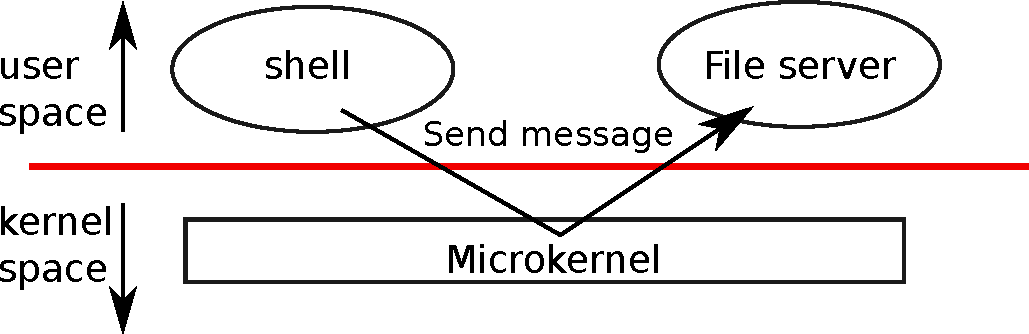
\includegraphics[scale=0.5]{fig/mkernel.pdf}
\caption{A microkernel with a file-system server}
\label{fig:mkernel}
\end{figure}

Figure~\ref{fig:mkernel}
illustrates this microkernel design.  In the figure, the file system runs as a
user-level process.  OS services running as processes are called servers.
To allow applications to interact with the
file server, the kernel provides an inter-process communication
mechanism to send messages from one
user-mode process to another.  For example, if an application like the shell
wants to read or write a file, it sends a message to the file server and waits
for a response. 

In a microkernel, the kernel interface consists of a few low-level
functions for starting applications, sending messages,
accessing device hardware, etc.  This organization allows the kernel to be 
relatively simple, as most of the operating system
resides in user-level servers.

In the real world, both monolithic kernels and microkernels are
popular. Many
Unix kernels are monolithic. For example, Linux has a monolithic kernel,
although some OS functions run as user-level servers (e.g., the windowing
system).  Linux delivers high performance to OS-intensive applications, partially
because the subsystems of the kernel can be tightly integrated.

Operating systems such as Minix, L4, and QNX are organized as a microkernel with
servers, and have seen wide deployment in embedded settings.  A
variant of L4, seL4, is small enough that it has been verified for
memory safety and other security properties~\cite{sel4}.

There is much debate among developers of operating systems which
organization is better, and there is no conclusive evidence one way or
the other.  Furthermore, it depends much on what ``better'' means:
faster performance, smaller code size, reliability of the kernel,
reliability of the complete operating system (inclusing user-level
services), etc.

There are also practical considerations that may be more important
than the question of which organization.  Some operating systems
have a microkernel but run some of the user-level services in kernel
space for performance reasons.  Some operating systems have monolithic
kernels because that is how they started and there is little incentive
to move to a pure microkernel organization, because new features may
be more important than rewriting the existing operating system to fit a microkernel
design.

From this book's perspective, microkernel and monolithic operating
systems share many key ideas.  They implement system calls, they use
page tables, they handle interrupts, they support processes, they use
locks for concurrency control, they implement a file system,
etc. This book focuses on these core ideas.

Xv6 is
implemented as a monolithic kernel, like most Unix operating systems.
Thus, the xv6 kernel interface corresponds to the operating system
interface, and the kernel implements the complete operating system.  Since 
xv6 doesn't provide many services, its kernel is smaller than some
microkernels, but conceptually xv6 is monolithic.  

\section{Code: xv6 organization}

\begin{figure}[t]
\center
\begin{tabular}{l|l}
{\bf File} & {\bf Description} \\
\midrule
bio.c & Disk block cache for the file system. \\
console.c & Connect to the user keyboard and screen. \\
entry.S & Very first boot instructions. \\
exec.c & exec() system call. \\
file.c & File descriptor support. \\
fs.c & File system. \\
kalloc.c & Physical page allocator. \\
kernelvec.S & Handle traps from kernel, and timer interrupts. \\
log.c & File system logging and crash recovery. \\
main.c & Control initialization of other modules during boot. \\
pipe.c & Pipes. \\
plic.c & RISC-V interrupt controller. \\
printf.c & Formatted output to the console. \\
proc.c & Processes and scheduling. \\
sleeplock.c & Locks that yield the CPU. \\
spinlock.c & Locks that don't yield the CPU. \\
start.c & Early machine-mode boot code. \\
string.c & C string and byte-array library. \\
swtch.S & Thread switching. \\
syscall.c & Dispatch system calls to handling function. \\
sysfile.c & File-related system calls. \\
sysproc.c & Process-related system calls. \\
trampoline.S & Assembly code to switch between user and kernel. \\
trap.c & C code to handle and return from traps and interrupts. \\
uart.c & Serial-port console device driver. \\
virtio\_disk.c & Disk device driver. \\
vm.c & Manage page tables and address spaces. \\
\end{tabular}
\caption{Xv6 kernel source files.}
\label{fig:source}
\end{figure}

The xv6 kernel source is in the {\tt kernel/} sub-directory. The
source is divided into files, following a rough notion of modularity;
Figure~\ref{fig:source} lists the files.  The inter-module interfaces
are defined in \lstinline{defs.h} \fileref{kernel/defs.h}.

%% 
\section{Process overview}
%% 

The unit of isolation in xv6 (as in other Unix operating systems) is a 
\indextext{process}.
The process abstraction prevents one process from wrecking or spying on
another process's memory, CPU, file descriptors, etc.  It also prevents a process
from wrecking the kernel itself, so that a process can't subvert the kernel's
isolation mechanisms.
The kernel must implement the process abstraction with care because
a buggy or malicious application may trick the kernel or hardware into doing
something bad (e.g., circumventing isolation).  The mechanisms used by
the kernel to implement processes include the user/supervisor mode flag, address spaces,
and time-slicing of threads.

To help enforce isolation, the process abstraction provides the
illusion to a program that it has its own private machine.  A process provides
a program with what appears to be a private memory system, or
\indextext{address space}, 
which other processes cannot read or write.
A process also provides the program with what appears to be its own
CPU to execute the program's instructions.

Xv6 uses page tables (which are implemented by hardware) to give each process
its own address space. The RISC-V page table
translates (or ``maps'') a
\indextext{virtual address}
(the address that an RISC-V instruction manipulates) to a
\indextext{physical address}
(an address that the CPU chip sends to main memory).

\begin{figure}[t]
\centering
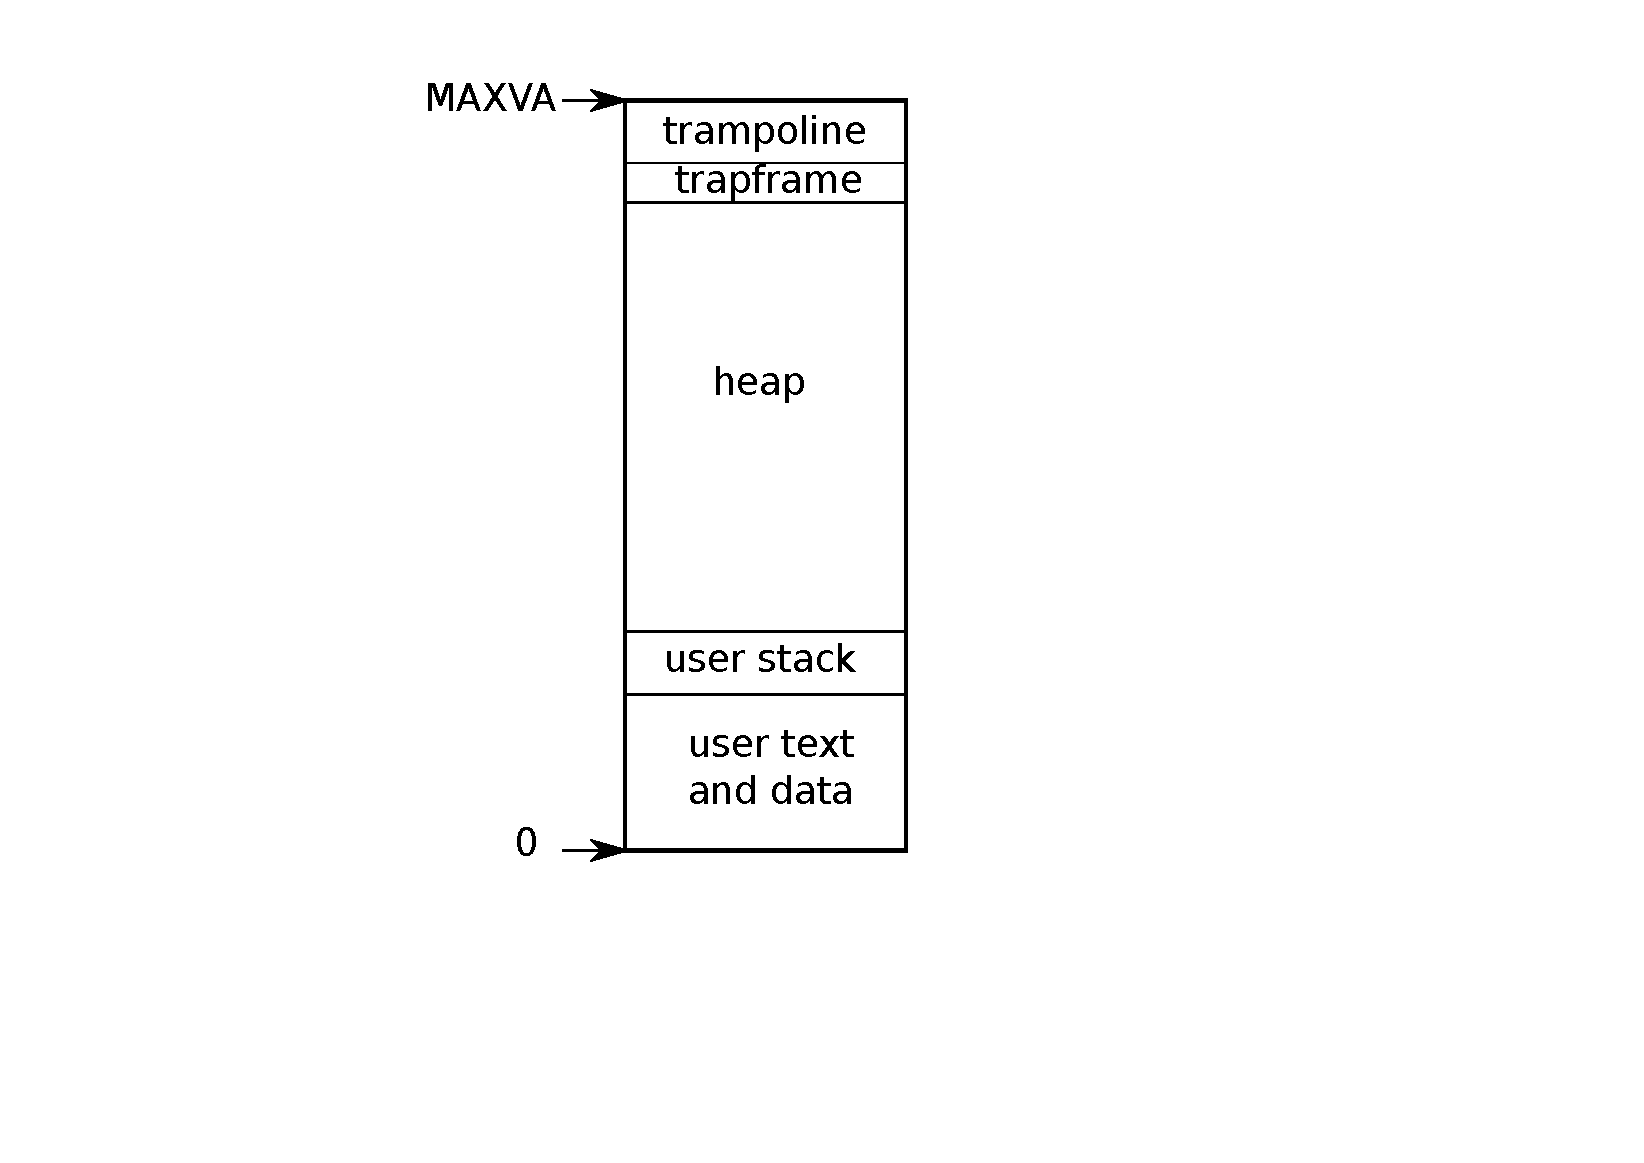
\includegraphics[scale=0.5]{fig/as.pdf}
\caption{Layout of a process's virtual address space}
\label{fig:as}
\end{figure}

Xv6 maintains a separate page table for each process that defines that process's
address space. As illustrated in 
Figure~\ref{fig:as},
an address space includes the process's
\indextext{user memory}
starting at virtual address zero. Instructions come first,
followed by global variables, then the stack,
and finally a ``heap'' area (for malloc)
that the process can expand as needed.
There are a number of factors that limit the
maximum size of a process's address space:
pointers on the RISC-V are 64 bits wide;
the hardware only uses the low 39 bits when
looking up virtual addresses in page tables;
and xv6 only uses 38 of those 39 bits.
Thus, the maximum address is $2^{38}-1$ =
0x3fffffffff, which is \lstinline{MAXVA}~\lineref{kernel/riscv.h:/MAXVA/}.
At the top of the address space xv6 reserves a page
for a \indextext{trampoline} and a page mapping
the process's \indextext{trapframe}
to switch to the kernel, as we will explain in Chapter~\ref{CH:TRAP}.

The xv6 kernel maintains many pieces of state for each process,
which it gathers into a
\indexcode{struct proc}
\lineref{kernel/proc.h:/^struct.proc/}.
A process's most important pieces of kernel state are its 
page table, its kernel stack, and its run state.
We'll use the notation
\indexcode{p->xxx}
to refer to elements of the
\lstinline{proc}
structure; for example,
\indexcode{p->pagetable} is a pointer to the process's page table.

Each process has a thread of execution (or 
\indextext{thread}
for short) that executes the process's instructions.
A thread can be suspended and later resumed.
To switch transparently between processes,
the kernel suspends the currently running thread and resumes another process's
thread.  Much of the state of a thread (local variables, function call return
addresses) is stored on the thread's stacks.
Each process has two stacks: a user stack and a kernel stack
(\indexcode{p->kstack}).
When the process is executing user instructions, only its user stack
is in use, and its kernel stack is empty.
When the process enters the kernel (for a system call or interrupt),
the kernel code executes on the process's kernel stack; while
a process is in the kernel, its user stack still contains saved
data, but isn't actively used.
A process's thread alternates between actively using its user stack
and its kernel stack. The kernel stack is separate (and protected from
user code) so that the kernel
can execute even if a process has wrecked its user stack.

A process can make a system call by executing the RISC-V \indexcode{ecall}
instruction. This instruction raises the hardware privilege level and
changes the program counter to a kernel-defined entry point.  The code
at the entry point switches to a kernel stack and executes the kernel
instructions that implement the system call.  When the system call
completes, the kernel switches back to the user stack and returns to
user space by calling the \indexcode{sret} instruction, which lowers
the hardware privilege level and resumes executing user instructions
just after the system call instruction.  A process's thread can
``block'' in the kernel to wait for I/O, and resume where it left off
when the I/O has finished.

\indexcode{p->state} 
indicates whether the process is allocated, ready
to run, running, waiting for I/O, or exiting.

\indexcode{p->pagetable}
holds the process's page table, in the format
that the RISC-V hardware expects.
xv6 causes the paging hardware to use a process's
\lstinline{p->pagetable}
when executing that process in user space.
A process's page table also serves as the record of the
addresses of the physical pages allocated to store the process's memory.
%% 
\section{Code: starting xv6, the first process and system call}
%% 
To make xv6 more concrete, we'll outline how the kernel starts and
runs the first process. The subsequent chapters will describe the
mechanisms that show up in this overview in more detail.

When the RISC-V computer powers on, it initializes
itself and runs a boot loader which is stored in read-only
memory.  The boot loader loads the xv6 kernel into memory.  Then, in
machine mode, the CPU executes xv6 starting at
\indexcode{_entry}
\lineref{kernel/entry.S:/^.entry:/}.
The RISC-V starts with paging hardware disabled:
virtual addresses map directly to physical addresses.

The loader loads the xv6 kernel into memory at physical address
\texttt{0x80000000}.
The reason it places the kernel at
\texttt{0x80000000}
rather than
\texttt{0x0}
is because the address range
\texttt{0x0:0x80000000}
contains I/O devices.

The instructions at
\lstinline{_entry}
set up a stack so that xv6 can run C code.
Xv6 declares space for an initial stack,
\lstinline{stack0},
in the file
\lstinline{start.c}
\lineref{kernel/start.c:/stack0/}.
The code at
\lstinline{_entry}
loads the stack pointer register
\texttt{sp}
with the address
\lstinline{stack0+4096},
the top of the stack, because the stack
on RISC-V grows down.
Now that the kernel has a stack,
\lstinline{_entry}
calls into C code at
\lstinline{start}
\lineref{kernel/start.c:/^start/}.

The function
\lstinline{start}
performs some configuration that is only allowed in
machine mode, and then switches to supervisor mode.
To enter supervisor mode, RISC-V
provides the instruction
\lstinline{mret}.
This instruction is most often used to return from
a previous call from supervisor mode to machine mode.
\lstinline{start} isn't returning from such a call, and
instead sets things up as if there had been one:
it sets the previous privilege mode to
supervisor in the register
\lstinline{mstatus},
it sets the return address to
\lstinline{main}
by writing
\lstinline{main}'s
address into
the register
\lstinline{mepc},
disables virtual address translation in supervisor mode
by writing
\lstinline{0}
into the page-table register
\lstinline{satp},
and delegates all interrupts and exceptions
to supervisor mode.

Before jumping into supervisor mode,
\lstinline{start}
performs one more task: it programs the clock
chip to generate timer interrupts.
With this housekeeping out of the way,
\lstinline{start}
``returns'' to supervisor
mode by calling
\lstinline{mret}.
This causes the program counter to change
to
\lstinline{main}
\lineref{kernel/main.c:/^main/}.

After
\lstinline{main}
\lineref{kernel/main.c:/^main/}  
initializes several devices and subsystems, 
it creates the first process by calling 
\lstinline{userinit}
\lineref{kernel/proc.c:/^userinit/}.
The first process executes a small program written in RISC-V assembly,
make makes the first system call in xv6.
\indexcode{initcode.S} 
\lineref{user/initcode.S:3} loads the number for the \lstinline{exec}
system call, \lstinline{SYS_EXEC}
\lineref{kernel/syscall.h:/exec/},
into
register {\tt a7},
and then calls \lstinline{ecall} to re-enter the kernel.

The kernel uses the number in register {\tt a7} in \lstinline{syscall}
\lineref{kernel/syscall.c:/^syscall/} to call the desired system call.
The system call table \lineref{kernel/syscall.c:/syscalls/} maps
\lstinline{SYS_EXEC} to \lstinline{sys_exec}, which the kernel
invokes.  As we saw in Chapter~\ref{CH:UNIX}, \indexcode{exec}
replaces the memory and registers of the current process with a new
program (in this case, \indexcode{/init}).

Once the kernel has completed 
\lstinline{exec},
it returns to user space in
the \lstinline{/init} process.
\lstinline{Init}
\lineref{user/init.c:/^main/}
creates a new console device file
if needed
and then opens it as file descriptors 0, 1, and 2.
Then it starts a shell on the console.
The system is up.
%% 
\section{Real world}
%% 

Most operating systems have adopted the process concept, and most
processes look similar to xv6's.  Modern operating systems, however,
support several threads within a process, to allow a single process to
exploit multiple CPUs.  Supporting multiple threads in a
process involves quite a bit of machinery that xv6 doesn't have,
including potential interface changes (e.g., Linux's
\lstinline{clone},
a variant of
\lstinline{fork}),
to control which aspects of
a process threads share.
%% 
\section{Exercises}
%%

\begin{enumerate}

\item Add a system call to xv6
  that returns the amount of free memory available.

% break *0x3ffffff000
% disas 0x3ffffff000,+8
% set disassemble-next-line auto
% x/i $pc
% break *0x3ffffff10e
% print/x $sepc
% print/x $pc

\end{enumerate}
